\documentclass[11pt]{article}
\usepackage{euscript}

\usepackage{amsmath,amssymb,bm}
\usepackage{amsthm}
\usepackage{amssymb}
\usepackage{epsfig}
\usepackage{xspace}
\usepackage{color}
\usepackage{url}
\usepackage{subfigure}
\usepackage{enumerate}

%%%%%%%  For drawing trees  %%%%%%%%%
\usepackage{tikz}
\usetikzlibrary{calc, shapes, backgrounds}

%%%%%%%%%%%%%%%%%%%%%%%%%%%%%%%%%
\setlength{\textheight}{9in}
\setlength{\topmargin}{-0.600in}
\setlength{\headheight}{0.2in}
\setlength{\headsep}{0.250in}
\setlength{\footskip}{0.5in}
\flushbottom
\setlength{\textwidth}{6.5in}
\setlength{\oddsidemargin}{0in}
\setlength{\evensidemargin}{0in}
\setlength{\columnsep}{2pc}
\setlength{\parindent}{0em}
%%%%%%%%%%%%%%%%%%%%%%%%%%%%%%%%%


\newcommand{\eps}{\varepsilon}

\renewcommand{\c}[1]{\ensuremath{\EuScript{#1}}}
\renewcommand{\b}[1]{\ensuremath{\mathbb{#1}}}
\newcommand{\s}[1]{\textsf{#1}}

\newcommand{\E}{\textbf{\textsf{E}}}
\renewcommand{\Pr}{\textbf{\textsf{Pr}}}

\title{Data Visualization Course Project Proposal}
\author{Zhuoyue Zhao, Ya Gao\\\{zyzhao, ygao\}@cs.utah.edu}
\date{}

\begin{document}
\maketitle

\paragraph{Basic Info.} Visualization for FDIC Failed Bank List

Group members:

Zhuoyue Zhao (u1065756), zyzhao@cs.utah.edu

Ya Gao (u1137971), ygao@cs.utah.edu

https://github.com/zzy7896321/dataviscourse-pr-fdicfailedbanks


\paragraph{Background and Motivation.}

We looked at the resources on the course web page and found this FDIC failed
bank list. FDIC (Federal Deposit Insurance Corporation) was created in 1933
to restore public confidence in banking during the Greate Depression in the
1930s.  It insures a depositor for up to \$250,000 in a FDIC member bank in
the event of a bank failure. FDIC usually find a bank that is willing to
acquire a failed bank so that the deposits are simply transferred to the new
bank. However, sometimes, it cannot find a acquiring bank and will send the
insured funds directly to the customers. It is amazing that no depositor has
ever lost FDIC insured funds since its establishment but it is also worrying
that a massive wave of bank failures or a large bank failure could fail FDIC.
We are curious about how reliable FDIC has been and will be in the future.

\paragraph{Project Objectives.} 
We plan to visualize the spatio-temporal FDIC bank failures as well as the
distribution of acquiring banks. 1) The primary goal is to get an idea about
how useful and reliable FDIC has been in the past. 2) We might also want to
know how likely will FDIC fail if a lot of bank or a large bank fails based on
the peak period of failure in history. 3) We want to use d3 and svg to create
the visualization. We also want to use brushing and linking to allow exploring
the details of the data.

\paragraph{Data.}
We downloaded a detailed list of FDIC failed banks from 1934. It can be
obtained by launching the select-all query at
\url{https://www5.fdic.gov/hsob/SelectRpt.asp?EntryTyp=30&Header=1}. It
includes the name, the location of the headquarter, the effective date, the
total deposits, the total assets and other data of the banks.

We also have a second list of FDIC failed banks from October 1, 2000, available
at \url{https://www.fdic.gov/bank/individual/failed/banklist.html}. In
addition to the data available in the first table, it also lists the acquiring
institutions of the failed banks.

\paragraph{Data Processing.}
The data in both tables are quite clean. There are a few missing values in
irrelevant columns and the estimated loss column. To deal with that, we'll
ignore those rows with missing values in the estimated loss column. There are
4095 records in the table, which might be too many for our purpose. We are
considering restricting the data to starting from October 1, 2000. We also
plan to do some aggregations over the data on the numeric columns grouped by
either year or state so that we can have a spatio-temporal summary of the
data. We can also compute the statistics of failed banks each acquiring
institutions acquired by joining the two table. That's the second reason why
we will restrict the data in the first table to the ones after October 1,
2000.

\paragraph{Visualization Design.} We proposed the following 3 prototype designs.

\begin{enumerate}[\textrm{Design} 1)]
    \item See Figure \ref{fig:design_1}.

        \begin{figure}[!h]
            \centering
            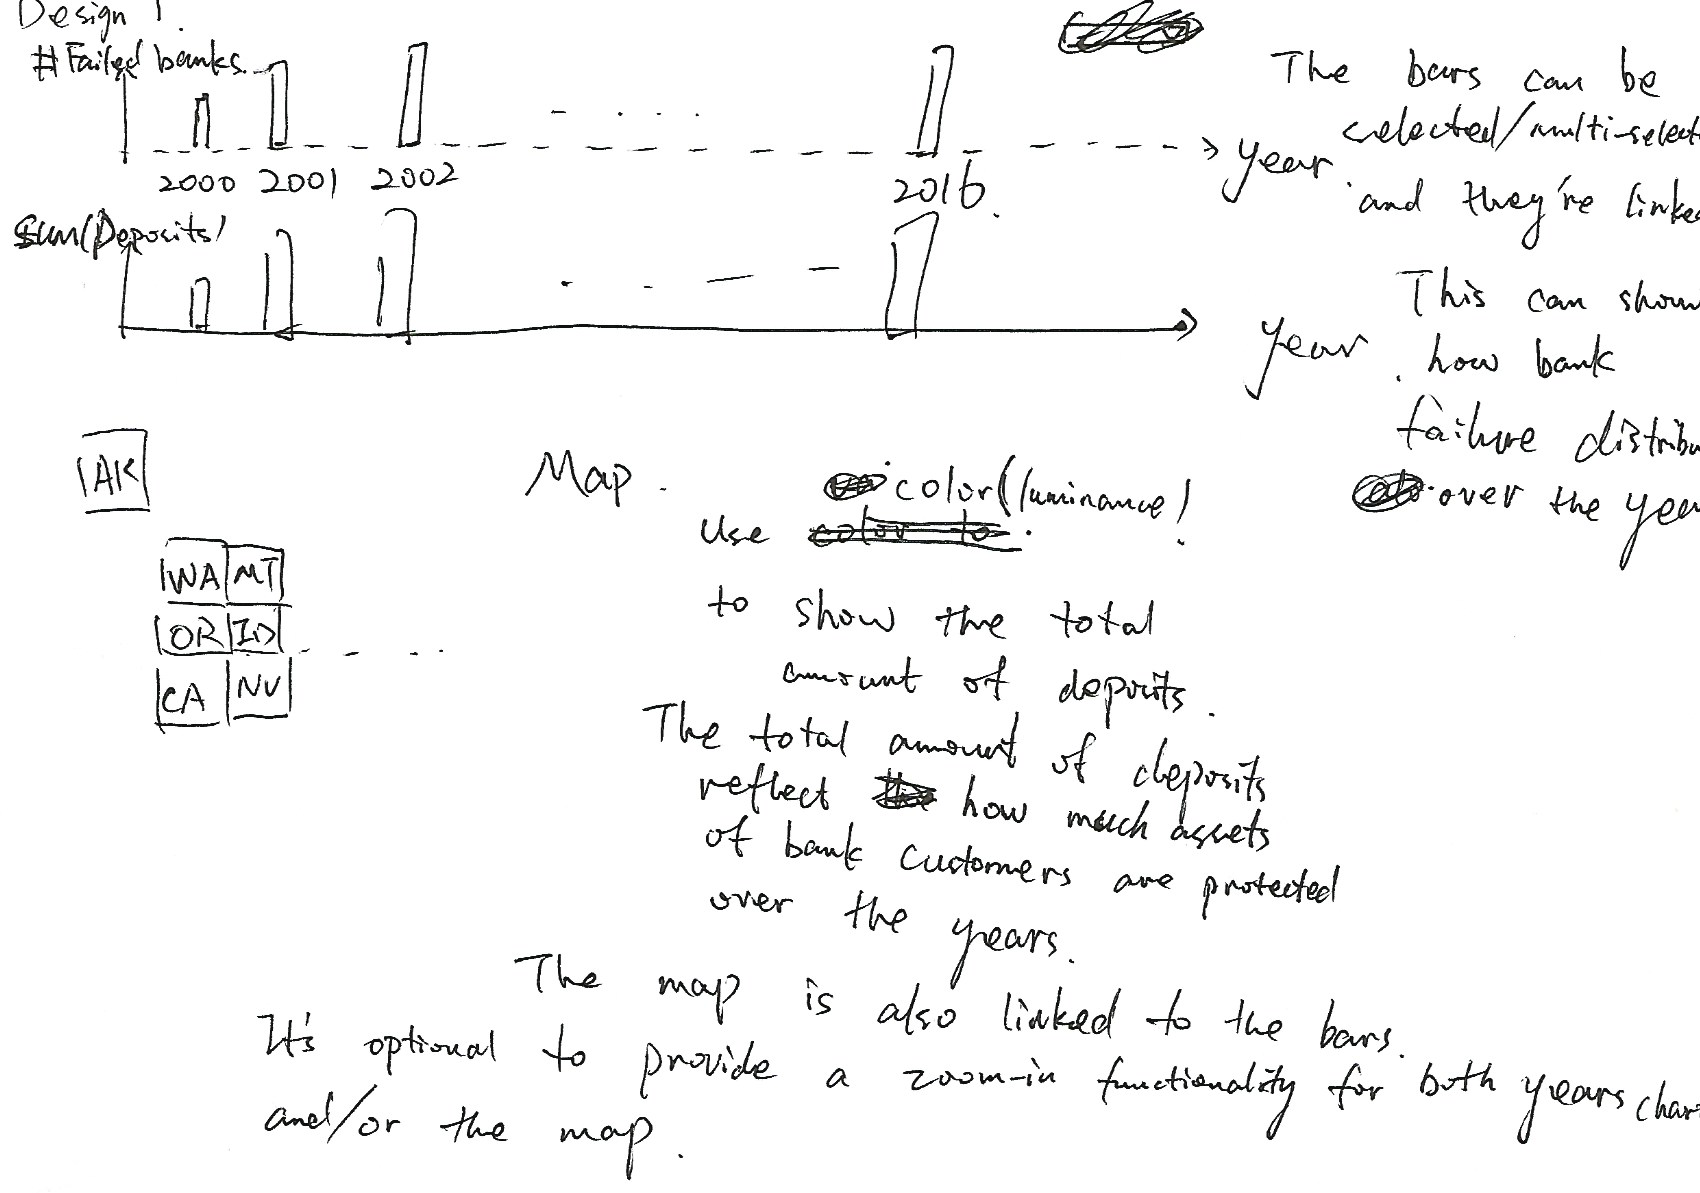
\includegraphics[width=0.9\textwidth]{fig/design_1}
            \caption{Design 1}
            \label{fig:design_1}
        \end{figure}

        Our first design consists of 3 charts: two yearly bar charts and a
        map. 
        
        The first bar chart is on the top, and plot the number of failed banks
        of each year from 2000 to 2016. The second bar chart is below the
        first one, and has the same x-axis. The y-axis is instead the
        summation of the total deposits in the failed banks in each year.
        These two bar charts show the failure distribution over the years in
        terms of both numbers and amounts. We anticipate that the two
        quantities are correlated but can vary a lot. For example, we expect
        the hike in the recent financial crisis from 2008 might be more
        obvious in the second bar chart since several large banks went
        bankcrupt.  The map uses color luminance to show the total amount of
        deposits of the failed banks in each state. It visualizes the spatial
        distribution of the failed banks.

        The bars in the first bar chart can be selected or multi-selected. The
        second bar chart and the map are linked to the first bar chart. The
        bars of the same years in the second bar charts are highlighted as in the
        first bar charts. The map is updated to display the sum of the selected years.

        An optional feature of this design is to provide a zoom-in feature for
        both the year charts and the map to allow exploration of the details
        at a lower granularity.

        The main advantage of this design is giving a summary of the failed
        banks and clearly shows the trends and distribution in both time and
        space. However, it lacks the ability to allow user to browse the
        details even if we have a zoom-in feature that allows the users to
        zoom-in to monthly charts or state maps.

    \item See Figure \ref{fig:design_2}.

        \begin{figure}[!h]
            \centering
            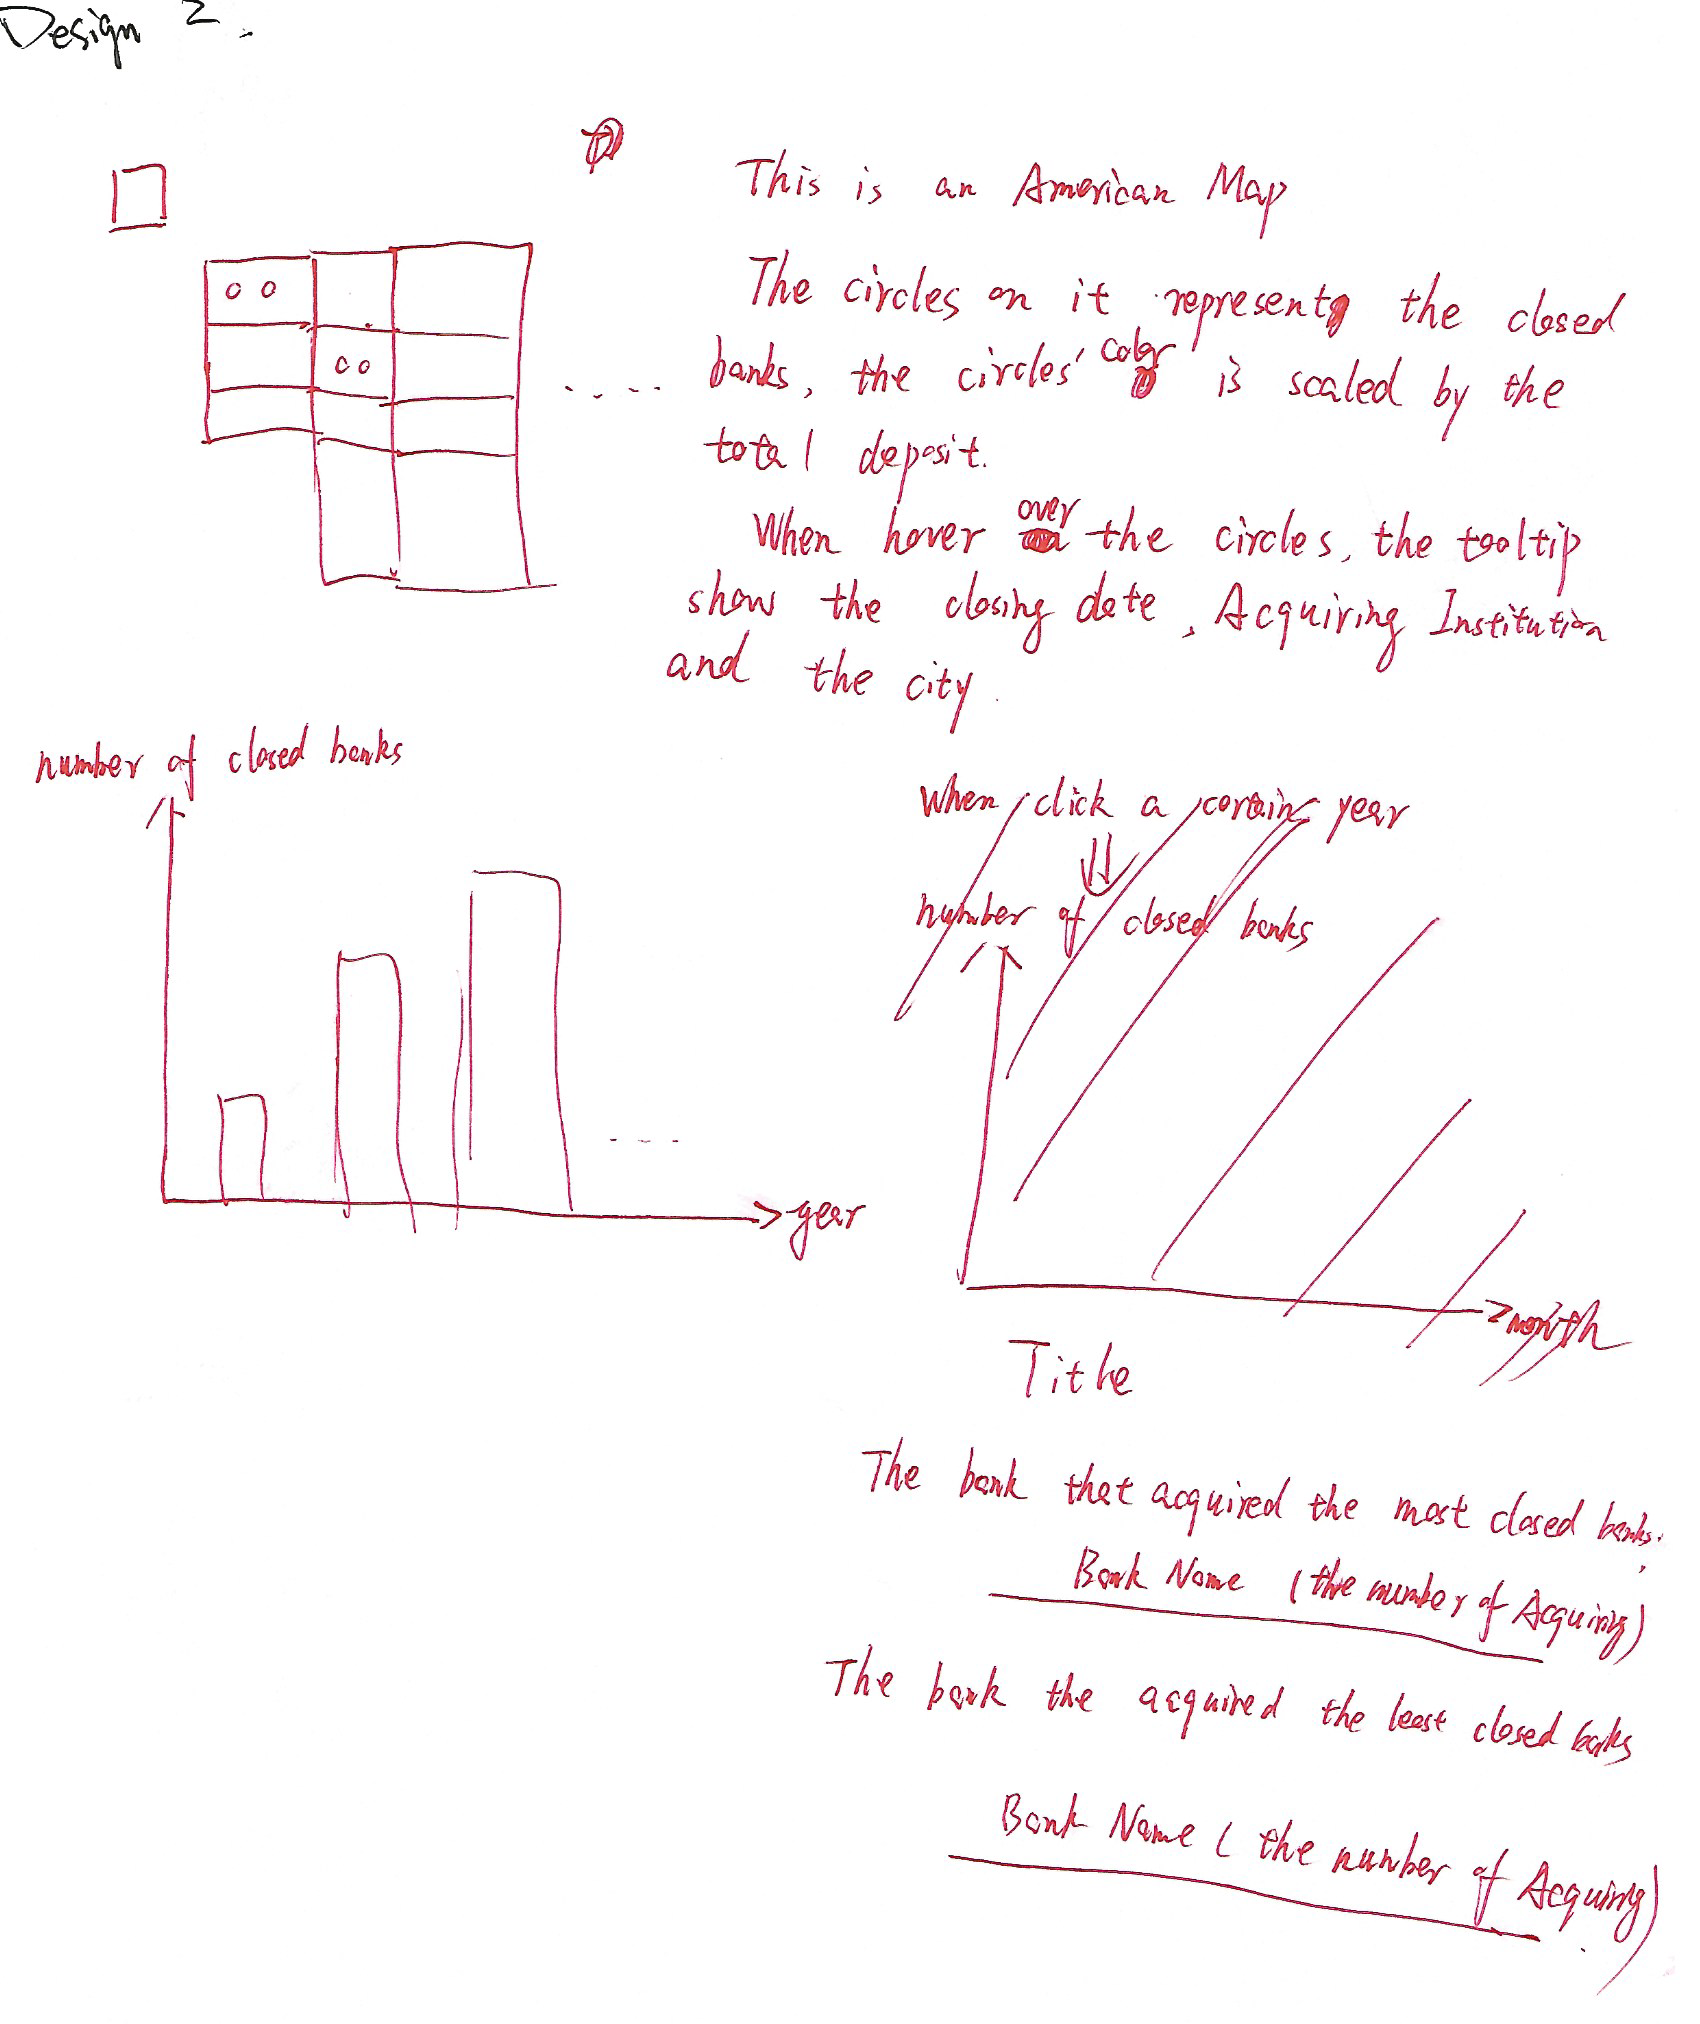
\includegraphics[width=0.9\textwidth]{fig/design_2}
            \caption{Design 2}
            \label{fig:design_2}
        \end{figure}

        The second design features a map, a bar chart and a list of top
        acquiring institutions.

        At the top of the page is a map of the states. In each state, there
        are circles that represents failed banks, whose color lumination is
        scaled according to the total deposit. When a user hover the mouse
        over a circle, a tooltip is shown with the details of the failed bank.

        Below the map are the bar chart ant the list. The bar chart on the
        left shows the number of failed banks over the years while the list on
        the right shows the top acquiring institions of the failed banks by
        the total number of failed banks they acquired over the years.

        This design enables browsing details of the failed banks. But the
        three visualization elements are unlinked. It's hard to use it to
        explore the data.

    \item See Figure \ref{fig:design_3}.
        
        \begin{figure}[!h]
            \centering
            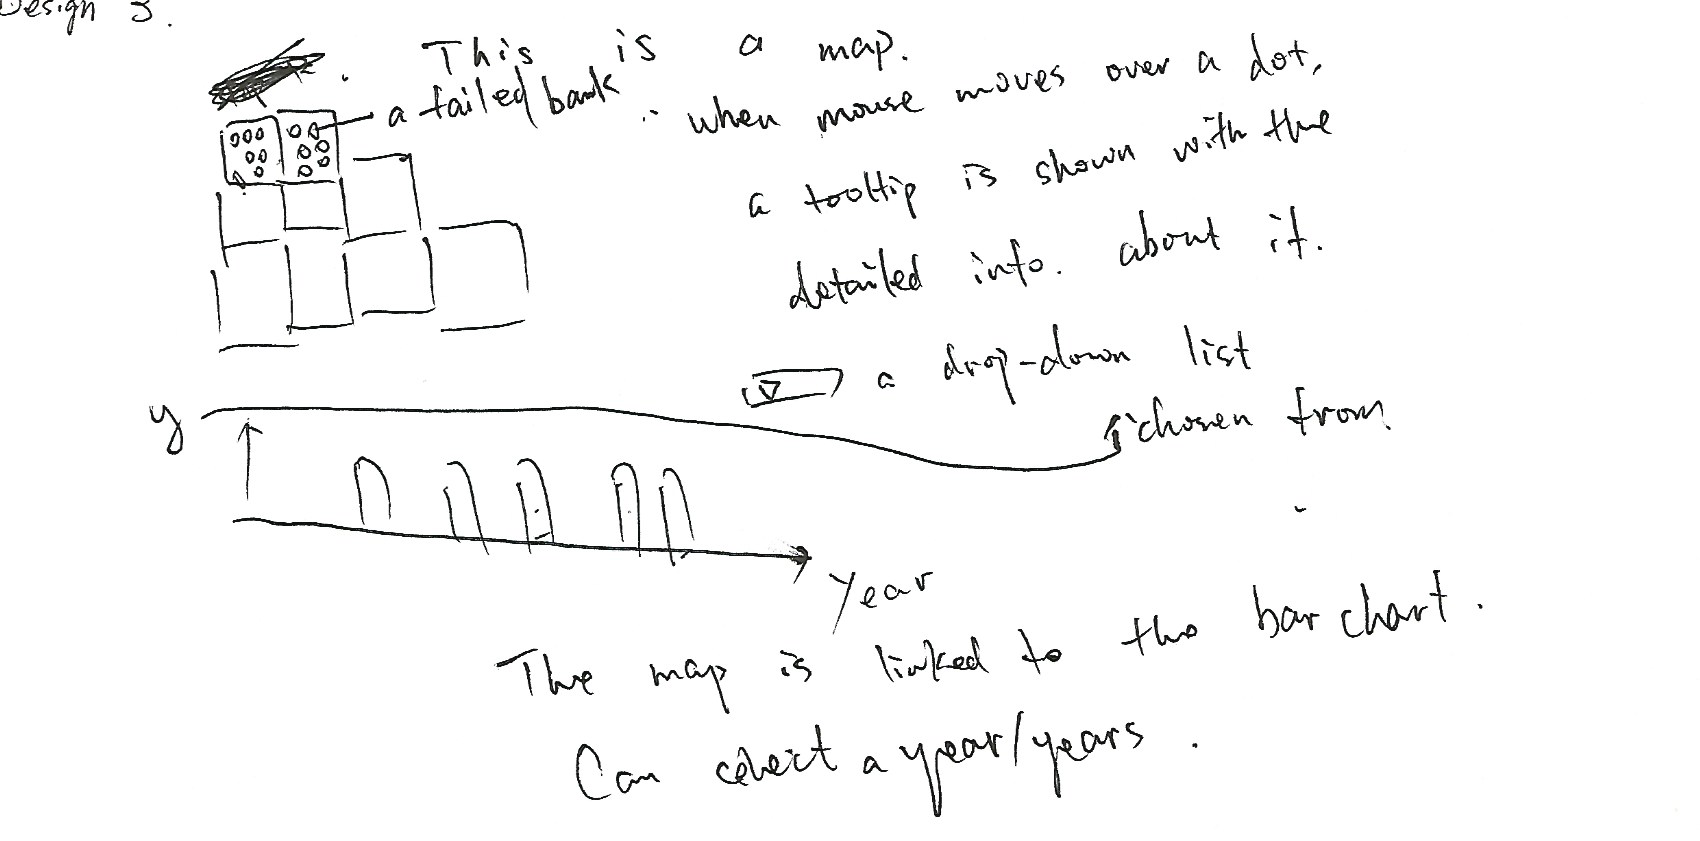
\includegraphics[width=0.9\textwidth]{fig/design_3}
            \caption{Design 3}
            \label{fig:design_3}
        \end{figure}

        The third design features a map, a bar chart with a configurable
        y-axis (through a drop-down list).

        The map, similar to that in design 2, plots the failed banks as
        circles in the states. The color luminance of the circles is scaled
        according to the total deposits of the failed banks. When the mouse
        hovers over a circle, the details of that bank is shown in a tooltip.

        The bar chart has year as its x-axis. The y-axis can be chosen in the
        drop-down list, including total deposits, number, total assets or
        estimated loss. This is more concise than the previous ones in the
        first chart and also shows different angles of the data.
        The bars in the bar chart can be selected as in design 1 and the map
        is also linked to the selections to reflect the selected years.
        
        This design combines the benefits of the previous two and also
        provides a cleaner and more intuitive visualization. However, it is
        not as easy as a line chart would be to see the trend in the bar
        chart. The placement of circles in the map is also hard because there
        might be multiple banks in the same state. Finally, it lacks the
        information of acquiring banks, which can give an idea of the roles of
        large banks and FDIC in the process of bank failure.

\end{enumerate}

After weighing the benefits and drawbacks of the ideas in each design, we
decided on the following final design (see Figure \ref{fig:final_design}).

\begin{figure}[!h]
    \centering
    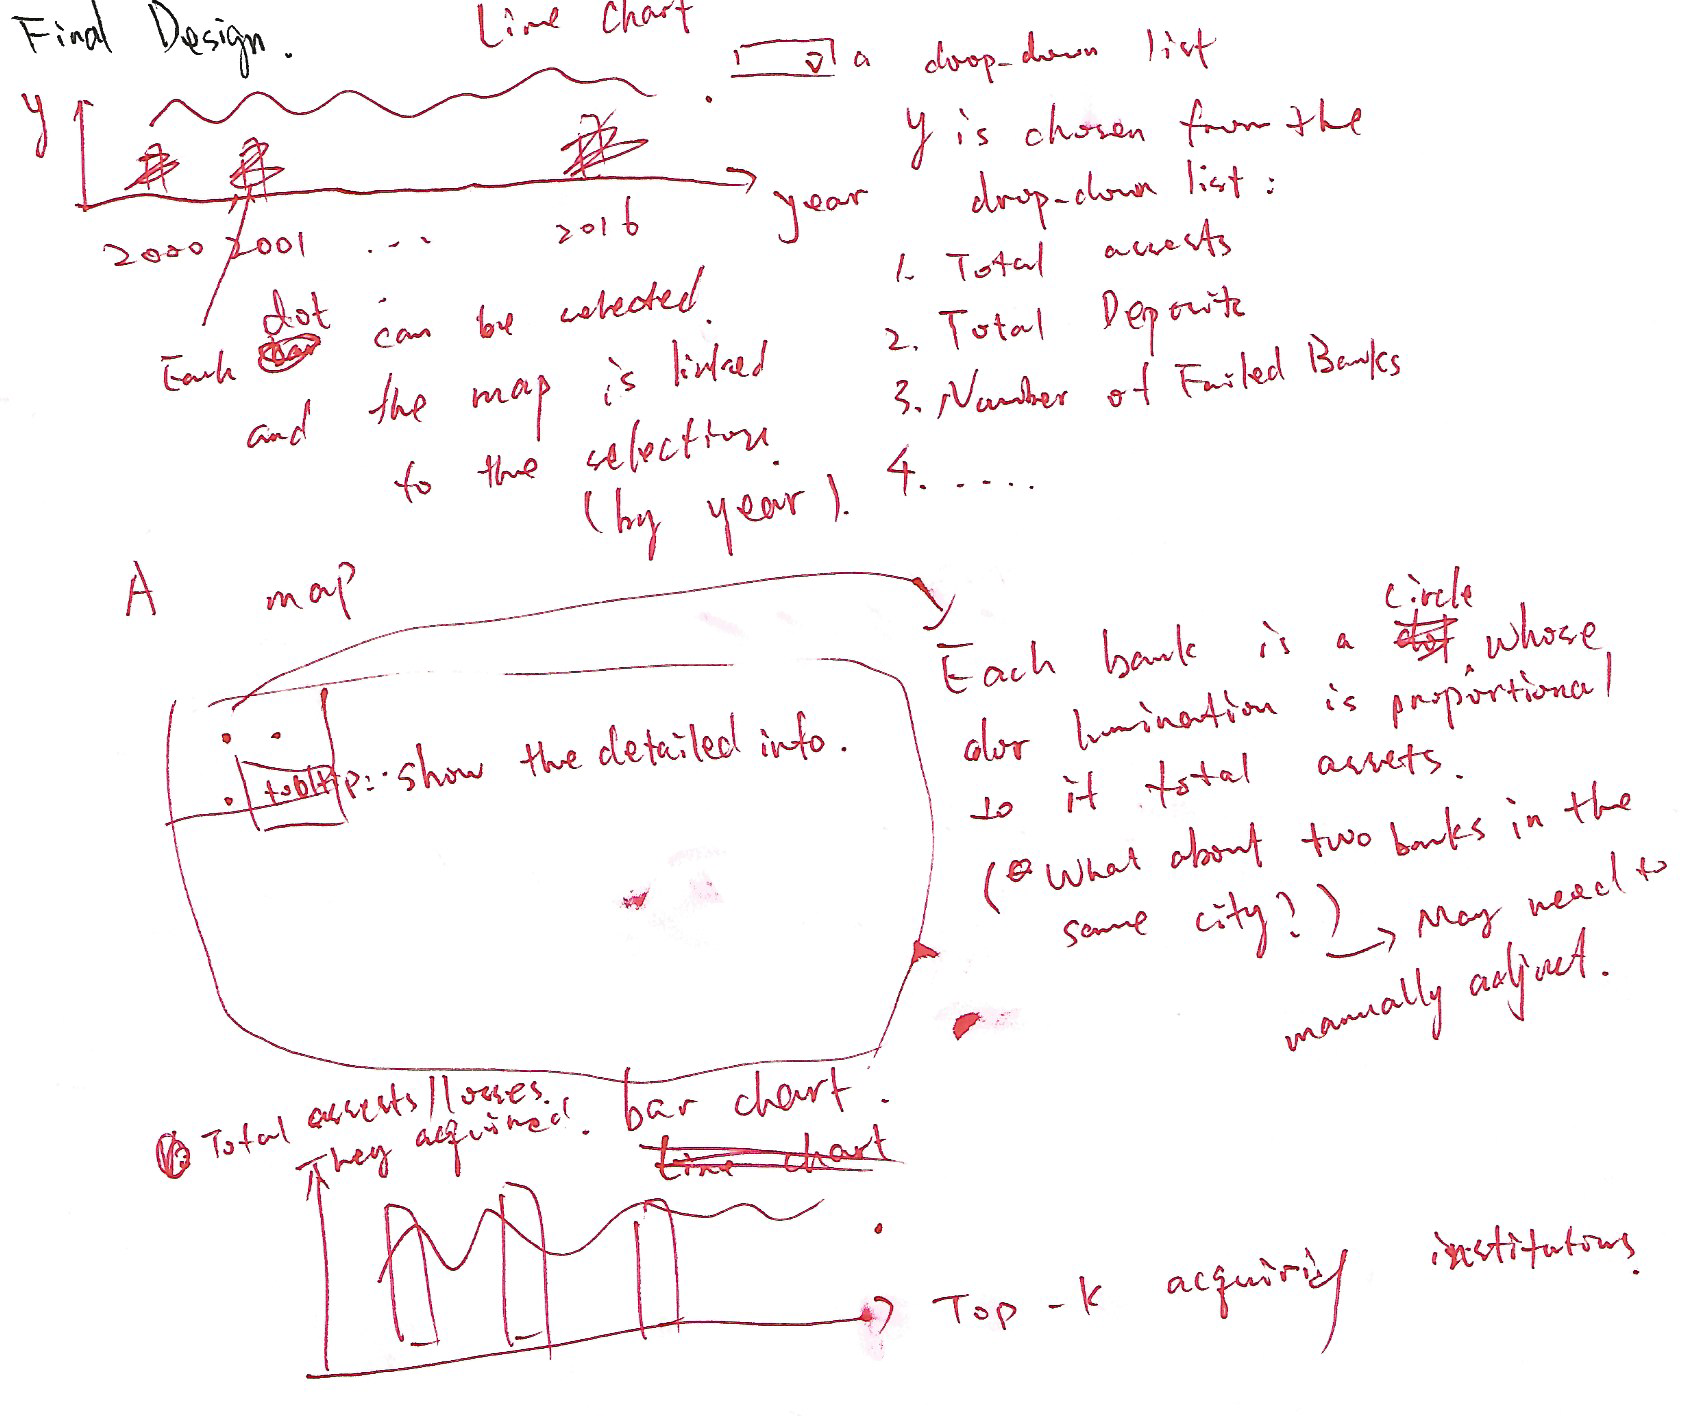
\includegraphics[width=0.9\textwidth]{fig/final_design}
    \caption{Final Design}
    \label{fig:final_design}
\end{figure}

The final design features a line chart, a map and a bar chart.

The line chart is similar to the bar chart in design 3. It has years as the
x-axis and a configurable y-axis through a drop-down list. The dots in the
year chart can be selected and the selection is linked to the other two
charts.

The map uses the map with the realistic shapes instead of square grids and
each bank is represented by a circle whose luminance is scaled according to
the total assets/deposits (TBD). The location of the dot is at the real
location of the headquarters of the failed bank. If multiple are in the same
city, they will be placed around that city. To achieve this, we can either
design an algorithm to automatically decide where to place the dots, or
preprocess the data by hand, or a combination of the two. Each dot also has a
tooltip that shows the detailed information about the failed bank. The dots
shown in the map will reflect the year selections.

The last chart is a bar chart that shows the top-k acquiring institutions and
the special case where there's no acquirer if it is not in the chart. The
y-axis is the total assets of the failed banks that a particular institution
acquired. This can show the ability of large banks and FDIC to acquire failed
banks and might be able to show how concentrate the acquirings are.

\paragraph{Must-Have Features.} The must have features include

\begin{itemize}
    \item A line chart that shows the aggregations over the years.

    \item A map that shows the spatial distribution of the failed banks.

    \item A bar chart that shows the top-k acquiring institutions.

    \item They are linked together and years can be selected by clicking the
        bars in the first bar chart.
\end{itemize}

\paragraph{Optional Features.} The optional features include

\begin{itemize}
    \item Zoom-in functionality on both year charts (into month chart)
         and the map (into state-level maps).

     \item Fancy animations.
\end{itemize}

\paragraph{Project Schedule.} $\quad$

\begin{center}
\begin{tabular}{l|p{10cm}}
    \hline
    Week & Task \\\hline
    Oct 30 - Nov 4 & Create a static html with empty divs. Start working on
    the charts. Zhuoyue will be responsible for the line chart and preparing
    the data. Ya will be responsible for plotting the map and the bar chart.
    \\\hline 
    Nov 6 - Nov 11 & Continue working on the charts and at least be able to
    show something on the webpage. Prepare the Project Milestone.\\\hline
    Nov 13 - Nov 24 & Continue working on the charts. \\\hline
    Nov 27 - Dec 1 & Finish everything, write the report and create the project
    screen-cast. \\\hline
\end{tabular}
\end{center}

\end{document}
